\documentclass[conference]{IEEEtran}
\IEEEoverridecommandlockouts
% The preceding line is only needed to identify funding in the first footnote. If that is unneeded, please comment it out.
\usepackage{cite}
\usepackage{amsmath,amssymb,amsfonts}
\usepackage{algorithmic}
\usepackage{graphicx}
\usepackage{textcomp}
\usepackage{xcolor}
\def\BibTeX{{\rm B\kern-.05em{\sc i\kern-.025em b}\kern-.08em
    T\kern-.1667em\lower.7ex\hbox{E}\kern-.125emX}}
\begin{document}

\title{PLFS: A Checkpoint Filesystem for Parallel Applications\\
%{\footnotesize \textsuperscript{*}Note: Sub-titles are not captured in Xplore and
%should not be used}
%\thanks{Identify applicable funding agency here. If none, delete this.}
}

\author{\IEEEauthorblockN{1\textsuperscript{st} Su'an Xia}
\IEEEauthorblockA{%\textit{dept. name of organization (of Aff.)} \\
%\textit{name of organization (of Aff.)}\\
Shanghai, China \\
xiasa@shanghaitech.edu.cn}
}

\maketitle

\begin{abstract}
Parallel log structured file system, PLFS, is designed for the problem that traditional data layout has poor performance due to the mismatching between the underlying file system. However, by remapping the original data layout into the one which is optimized for the underlying file system, we can achieved a much better performance in bandwidth,
\end{abstract}

\begin{IEEEkeywords}
High performance computing, parallel computing, checkpointing, parallel file systems and IO
\end{IEEEkeywords}

\section{Introduction}
Applications can avoid the loss of failure by restating from the recent checkpoint which periodically saves the state of the application. However, it has become a bigger workload for file systems. The larger the supercomputer is, the bigger the workload is. Moreover, different checkpointing patterns can result in different difficulty.
\\Based on the fact, we developed a new approach 'PLFS', which is an interposition layer remapping the original data layout into the one which is optimized for the underlying file system.
\\Finally, we test the performance of PLFS and we find that writing to the underlying parallel file system through PLFS improves checkpoint bandwidth. What is more, PLFS is an optional mount point. It means that we can speed up without changing the original application.


\section{Design of an Interposition Layer}

There are 3 different checkpoint patterns: N-N, N-1 segmented and N-1 strided as showned in Figure 1. PLFS works as an interposition layer to remap an N-1 strided checkpoint pattern into an N-N checkpoint pattern. Therefore we can decrease the checkpoint time due to the increased bandwidth brought by N-N checkpoint pattern.
\\PLFS is a virtual FUSE file system. It is between the application and the underlying file system. It focuses on the remapping because it can make the most of many services provided by the underlying file system.
\\PLFS is designed specifically for large parallel N-1 checkpoint files. Its basic architecture is illustrated in Figure 2.

\begin{figure}[htbp]
	\centering
	\includegraphics[width=10cm,height=4cm]{pattern.png}
	\caption{Checkpoint patterns}
\end{figure}

\begin{figure}[htbp]
	\centering
	\includegraphics[width=10cm,height=8cm]{architecture.png}
	\caption{PLFS basic architecture}
\end{figure}

\subsection{Basic operation}
PLFS works as follow: PLFS creates a container structure which has a top-level directory called checkpoint1 and several sub-directories to store the application's data.
\\When process opens a file, PLFS will create a data file and a index file within a same sub-directory at the same time. What is more, the index file is shared by all processes on the compute node. 
\\When process writes a file, PLFS will write the data into the corresponding data file. Meanwhile PLFS will make a record in the corresponding index file which will record the length of the write, logical offset and a pointer to physical offset.
\\When process reads a file, PLFS will aggregate index files to create a lookup table. And for shorter query time, PLFS will record some other useful data.
\subsubsection{Reading from PLFS}
With the improvement in write, however, PLFS will have additional complexity for reads. When cached metadata is not available, constructing a global index by aggregating index files into a lookup table will have severy difficulty.
\\One difficulty is the concurrent writing with same offset of multiple processes.
Multiple processes in a uniform restart may not always read from a shared file sequentially due to timing differences between the write and read phases.
\\We choose FUSE to develop PLFS due to the transparency and simpleness. Of course it will add FUSE some additional overhead.
\subsubsection{Container Implementation}
To make the most of underlying parallel file system, the container has the same logical name as the PLFS file. Therefore it is eay for PLFS to pass a readdir system call or a mkdir system call to the underlying file system without any translation. Besides, due to the features of SUID bit, we use it to distinguish between regular directories and containers for correctness.
\\One difficulty stems from synchronized checkpointing. More specifically, if PLFS tries to create the same container concurrently bacause of multiple writes, this race condition will cause some unexpected errors. So to avoid this, we first make a hidden container with a unique name for each PLFS, then atomically rename it to the original container name.
\subsection{Metadata Operations}
Metadata Operations include accessing permissions (like SUID), capacity, the offset of last byte and the timestamp of last update.
\\Because the SUID bit on the container indicates that the directory is a regular directory or a container, we need an another file, the access file, to represent the appropriate SUID bit and other permissions relevant to the container. Capacity of the logical file is the sum of the capacities of files inside the container. The offset of the last byte is the maximum logical offset recorded in index files. The last update timestamp is the maximum of the last update timestamps.
\\Different from the assumption that these metadat are provided by the underlying file system, these metadata are computed from the underlying files within the container.
\\However, calculating with stat call is expensive, we can cache recently computed values in the metadata subdirectory to reduce the number of stat calls and then speed up this process.  So when the last writer on certain node closes the file, we cache all the information in memory data structures into metadata subdirectory.
\\If no process has this container open for writing, then a stat call on the container issues a readdir on the metadata subdirectory, then reports all the metadata. If exist writing, we create a file in the openhosts subdirectory named by its hostname if process on that node tries to write, which will indicate modified files to avoid old metadata. Then we readdir both openhosts and metadata subdirectory to generate the finally updated correct metadata.

\section{Evaluation}
The following are some test results using the LANL synthetic checkpoint tool, MPI-IO Test. We will give a brief results evluation.
\subsection{MPI-IO Test}
Firstly we will show the relationship  between bandwidth or time and the number of processes. As shown in Figure 3, we can see that the bandwidth goes up from 1 to 2 but goes down from 2 to 4. And the read bandwidth is larger then write bandwidth. I think it is ok because we only test 1,2,4 processes but in the paper he got the conclusion after testing much more processes. So any result is acceptable. In Figure 4, it is not hard to see that it costs more time as we increase the number of processes. It is predicted.
\\Then let us compare the bandwidth and time between PLFS and the underlying file system. In Figure 5, we can see that PLFS greatly increases the read bandwidth because of metadata. However write bandwidth is similar to the original one. I think it is because of the optimization of the original file system or we test too few processes. In figure 6, we can see that we only get a little speedup in read. 
\\Above all, we test in the condition that 128K in size and 1024 in nobj.
\\In terms of \textit{size} and \textit{nobj}, we also make sone tests and draw some simple conclusions. For nobj, it easy to find that bandwidth goes up when nobj gets larger. So is the time spent. However there is no obvious relationship between bandwidth and size.

\section{Summary of lessons}
\paragraph{Supercomputer} The file system is more important in supercomputer. 
\paragraph{Interposition layer} Sometimes, a transition rather than direct may get a better result.
\paragraph{Race condition} In file system we should consider race condition any time. And try to avoid them is inevitable.
\paragraph{openmpi} I get familiar with it and its argument.
\paragraph{Flow chart} I learned how to read the source code.
\paragraph{Piazza} Piazza is no.1.

\begin{figure}
	\centerline{
	\includegraphics[width=9cm,height=5cm]{Bandwidth_PLFS.png}}
	\caption{Bandwidth under PLFS}
\end{figure}

\begin{figure}
	\centerline{
	\includegraphics[width=9cm,height=5cm]{Time_PLFS.png}}
	\caption{Time under PLFS}
\end{figure}

\begin{figure}
	\centerline{
	\includegraphics[width=9cm,height=5cm]{Bandwidth_Compare.png}}
	\caption{Bandwidth compare between PLFS and underlying file system}
\end{figure}

\begin{figure}
	\centerline{
	\includegraphics[width=9cm,height=5cm]{Time_Compare.png}}
	\caption{Time compare between PLFS and underlying file system}
\end{figure}

\begin{figure*}
	\centerline{
		\includegraphics[scale=0.8]{open.eps}}
	\caption{Open flow chart}
\end{figure*}
\begin{figure*}
	\centerline{
		\includegraphics[scale=0.8]{close.eps}}
	\caption{Close flow chart}
\end{figure*}
\begin{figure*}
	\centerline{
		\includegraphics[scale=0.8]{read.eps}}
	\caption{Read flow chart}
\end{figure*}
\begin{figure*}
	\centerline{
		\includegraphics[scale=0.8]{write.eps}}
	\caption{Write flow chart}
\end{figure*}
\end{document}
